\documentclass[tikz, border = 0.1cm]{standalone}
\usepackage{tikz}
\usetikzlibrary{bayesnet}
\usepackage{amsmath, amsthm, amssymb, amsfonts}
\tikzset{>=latex}

\begin{document}
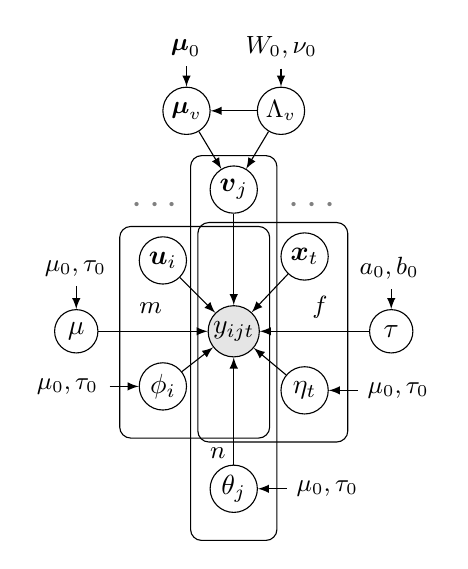
\begin{tikzpicture}

\node[circle, draw = black, fill = gray!20, inner sep = 0pt, minimum size = 0.65cm] (obs) at (0, 0) {{$y_{ijt}$}};
\node[circle, draw = black, inner sep = 0pt, minimum size = 0.6cm] (ui) at (-0.9, 0.9) {{$\boldsymbol{u}_{i}$}};
\node[circle, draw = black, inner sep = 0pt, minimum size = 0.6cm] (vj) at (0, 1.8) {{$\boldsymbol{v}_{j}$}};
\node[circle, draw = black, inner sep = 0pt, minimum size = 0.6cm] (xt) at (0.9, 0.95) {{$\boldsymbol{x}_{t}$}};
\node[circle, draw = black, inner sep = 0pt, minimum size = 0.6cm] (phi) at (-0.9, -0.7) {{$\phi_{i}$}};
\node[circle, draw = black, inner sep = 0pt, minimum size = 0.6cm] (theta) at (0, -2) {{$\theta_{j}$}};
\node[circle, draw = black, inner sep = 0pt, minimum size = 0.6cm] (eta) at (0.9, -0.75) {{$\eta_{t}$}};
\node[circle, draw = black, inner sep = 0pt, minimum size = 0.55cm] (tau) at (2, 0) {{$\tau$}};
\node[circle, draw = black, inner sep = 0pt, minimum size = 0.55cm] (mu) at (-2, 0) {{$\mu$}};

\foreach \n in {ui, vj, xt, tau, mu, phi, theta, eta}{\path [draw, ->] (\n) edge (obs);}

\node [text width = 0.2cm] (m) at (-1.1, 0.3) {\small{$m$}};
\plate[] {plate1} {(obs) (ui) (m) (phi)} { };
\node [text width = 0.6cm] (n) at (0, -1.55) {\small{$n$}};
\plate[] {plate2} {(obs) (vj) (n) (theta)} { };
\node [text width = 0.2cm] (f) at (1.1, 0.3) {\small{$f$}};
\plate[] {plate3} {(obs) (xt) (f) (eta)} { };

\node[circle, draw = black, inner sep = 0pt, minimum size = 0.6cm] (muv) at (-0.6, 2.8) {\small{$\boldsymbol{\mu}_{v}$}};
\node[circle, draw = black, inner sep = 0pt, minimum size = 0.6cm] (lambdav) at (0.6, 2.8) {\small{$\Lambda_{v}$}};
\node[text width = 0.8cm] (gamma) at (2, 0.8) {\small{$a_0,b_0$}};
\node[text width = 0.8cm] (hyper1) at (-2, 0.8) {\small{$\mu_{0},\tau_{0}$}};
\node[text width = 0.8cm] (hyper2) at (1.2, -2) {\small{$\mu_{0},\tau_{0}$}};
\node[text width = 0.8cm] (hyper3) at (2.1, -0.75) {\small{$\mu_{0},\tau_{0}$}};
\node[text width = 0.8cm] (hyper4) at (-2.1, -0.7) {\small{$\mu_{0},\tau_{0}$}};
\node[text width = 0.4cm] (mu0) at (-0.6, 3.6) {\small{$\boldsymbol{\mu}_{0}$}};
\node[text width = 0.9cm] (wnu0) at (0.6, 3.6) {\small{$W_{0},\nu_{0}$}};
\node[text width = 0.6cm] (cdots1) at (-1, 1.6) {\Large\color{gray}{$\cdots$}};
\node[text width = 0.6cm] (cdots2) at (1, 1.6) {\Large\color{gray}{$\cdots$}};

\path [draw, ->] (muv) edge (vj);
\foreach \n in {vj, muv}{\path [draw, ->] (lambdav) edge (\n);}
\path [draw, ->] (mu0) edge (muv);
\path [draw, ->] (wnu0) edge (lambdav);
\path [draw, ->] (gamma) edge (tau);
\path [draw, ->] (hyper1) edge (mu);
\path [draw, ->] (hyper2) edge (theta);
\path [draw, ->] (hyper3) edge (eta);
\path [draw, ->] (hyper4) edge (phi);

\end{tikzpicture}
\end{document}
